%!TEX root = ../dissertation.tex

\chapter{Tests and Results} \label{cha:test}

%%The purpose of this project is to show how a proto-AGI system such as OpenCog can be used 

\begin{table}[htbp]
  \centering
  \caption{Tabella Approcci}\label{Approcci}
  \medskip
\begin{tabular}{cccccccc}
\toprule
& \multicolumn{7}{c}{\textbf{Approcci}} \\
\textbf{Dati di Input} &  \textbf{1°} &  \textbf{1°} &  \textbf{1°}  &  \textbf{2°}  &  \textbf{3°}  &  \textbf{4°}  &  \textbf{5°}  \\
\midrule
\rowcolor{gray!45}
Depth & \checkmark & & & \checkmark & & \checkmark & \checkmark \\
Conf & & \checkmark & & \checkmark & & \checkmark & \checkmark \\
\rowcolor{gray!45}
Color - R & & & &  & \checkmark  & \checkmark & \checkmark \\
Color - G & & & &  & \checkmark  & \checkmark & \checkmark \\
\rowcolor{gray!45}
Color - B & & & &  & \checkmark  & \checkmark & \checkmark \\
Grey-Scale & & & \checkmark & \checkmark & & & \\
\bottomrule
\end{tabular}
\end{table}

\begin{figure} [h]
\centering
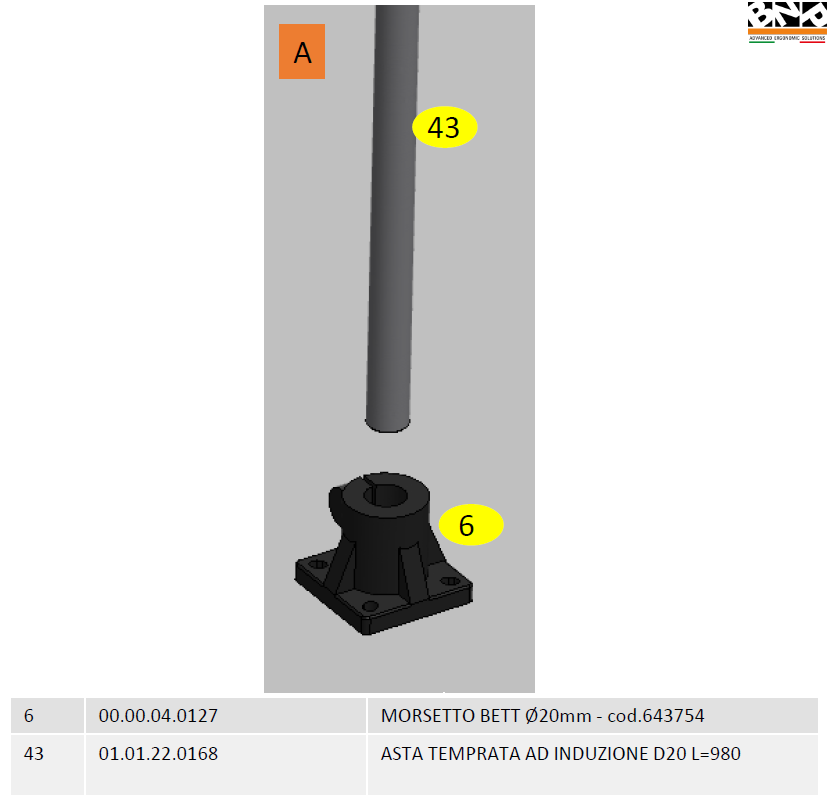
\includegraphics[width=1.0
\textwidth]{figures/Magistrale/ass_obj_1}
\caption[BFS Example]{
\label{fig:ass_obj_1}}
\end{figure} 

\begin{figure} [h]
\centering
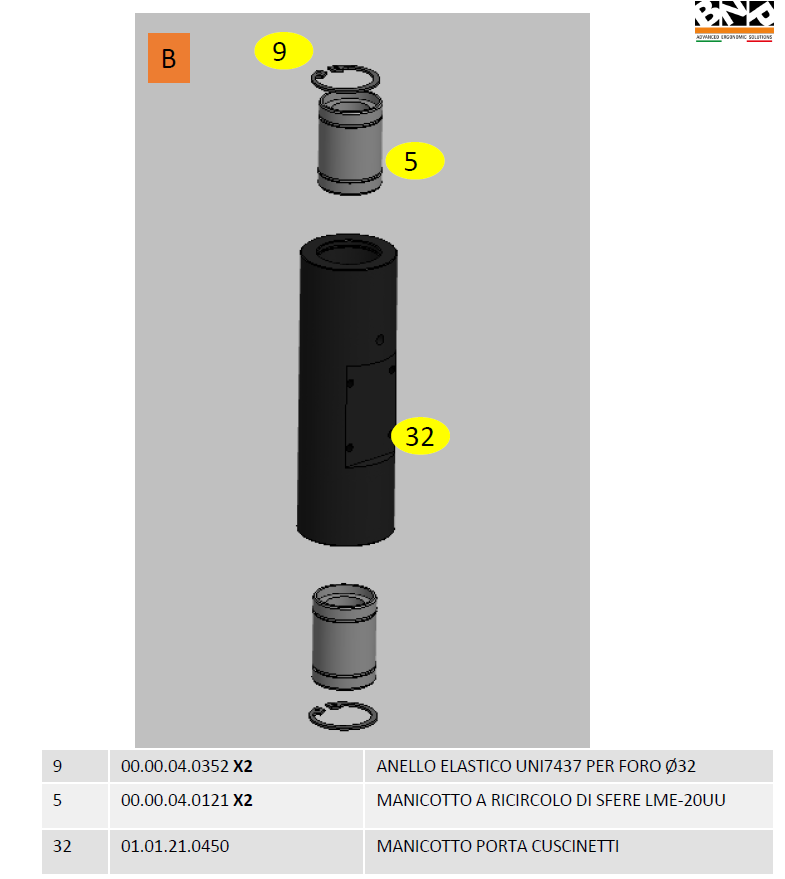
\includegraphics[width=1.0
\textwidth]{figures/Magistrale/ass_obj_2}
\caption[BFS Example]{
\label{fig:ass_obj_2}}
\end{figure} 

\begin{figure} [h]
\centering
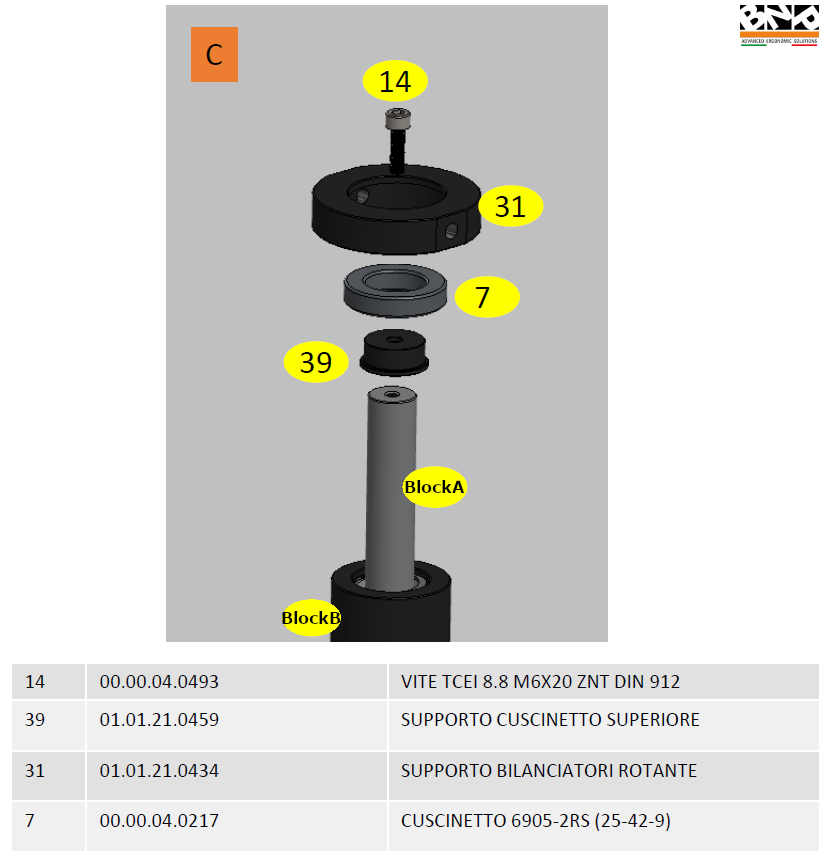
\includegraphics[width=1.0
\textwidth]{figures/Magistrale/ass_obj_3}
\caption[BFS Example]{
\label{fig:ass_obj_3}}
\end{figure} 